%%%%%%%%%%%%%%%%%%%%%%% file template.tex %%%%%%%%%%%%%%%%%%%%%%%%%
%
% This is a general template file for the LaTeX package SVJour3
% for Springer journals.          Springer Heidelberg 2010/09/16
%
% Copy it to a new file with a new name and use it as the basis
% for your article. Delete % signs as needed.
%
% This template includes a few options for different layouts and
% content for various journals. Please consult a previous issue of
% your journal as needed.
%
%%%%%%%%%%%%%%%%%%%%%%%%%%%%%%%%%%%%%%%%%%%%%%%%%%%%%%%%%%%%%%%%%%%
%
% First comes an example EPS file -- just ignore it and
% proceed on the \documentclass line
% your LaTeX will extract the file if required
\begin{filecontents*}{example.eps}
%!PS-Adobe-3.0 EPSF-3.0
%%BoundingBox: 19 19 221 221
%%CreationDate: Mon Sep 29 1997
%%Creator: programmed by hand (JK)
%%EndComments
gsave
newpath
  20 20 moveto
  20 220 lineto
  220 220 lineto
  220 20 lineto
closepath
2 setlinewidth
gsave
  .4 setgray fill
grestore
stroke
grestore
\end{filecontents*}
%
\RequirePackage{fix-cm}
%
\documentclass[natbib]{svjour3}                     % onecolumn (standard format)
%\documentclass[smallcondensed]{svjour3}     % onecolumn (ditto)
%\documentclass[smallextended]{svjour3}       % onecolumn (second format)
%\documentclass[twocolumn, natbib]{svjour3}          % twocolumn
%
\smartqed  % flush right qed marks, e.g. at end of proof
%
\usepackage{graphicx}
%
\usepackage{mathptmx}      % use Times fonts if available on your TeX system
%
% insert here the call for the packages your document requires
%\usepackage{latexsym}
% etc.
%
%\usepackage{natbib} % [numbers]
\usepackage{hyperref}



\usepackage{booktabs}
\usepackage{multirow}
\usepackage{tabularx}
\usepackage{longtable}
\usepackage{lipsum}
\usepackage{lscape}
\usepackage{siunitx}
\usepackage{amsmath}
\usepackage{rotating}
%\usepackage{cleveref}
% please place your own definitions here and don't use \def but
% \newcommand{}{}
%
% Insert the name of "your journal" with
\journalname{Energy Efficiency}
%
\begin{document}

\title{Performance Degradation Identification for Compressed Air Systems Using a Hybrid Machine Learning and Knowledge Based Fault Detection and Diagnostic System\thanks{This work was funded by Marine Renewable Energy Ireland (MaREI) at University College Cork}
}
%\subtitle{Do you have a subtitle?\\ If so, write it here}

%\titlerunning{Short form of title}        % if too long for running head

\author{Blinded Manuscript%etc.
}

%\authorrunning{Short form of author list} % if too long for running head

\institute{Blinded Manuscript
 %          S. Author \at
  %            second address
}

\date{Received: date / Accepted: date}
% The correct dates will be entered by the editor


\maketitle

\begin{abstract}
A rule based expert system for compressed air system fault detection and operational performance management is presented. The expert rule set takes a qualitative model based approach to fault detection, relying on fundamental engineering principles to detect when the compressed air system is not performing as expected. K-means clustering on the compressor power consumption is employed for mode identification and intelligent efficiency monitoring. The system is formally coded in MATLAB with a GUI for visualisation. The tool has been trialled on a compressed air system which is representative of installations in global industry. Successful determination of the system's operating mode was achieved. The rule set of 15 rules indicated that 9 faults were recurrent in the test case data set. Each of the symptoms which resulted in the rules highlighting a fault had two potential causes or diagnoses. Manual verification of which fault is actually present is currently required, with future refinement of the system planned allowing definitive diagnoses of faults detected. 
\keywords{Fault detection \and Clustering \and Compressed Air \and Expert Systems  \and Mode Identification \and Energy Efficiency}
% \PACS{PACS code1 \and PACS code2 \and more}
% \subclass{MSC code1 \and MSC code2 \and more}
\end{abstract}

\section{Introduction}
\label{intro}

In 2012 industry consumed 2,542 Mtoe of energy globally, which represented  over 28\% of the 8,980 Mtoe of global final energy consumption (\cite{IEA2012}). In an Irish context, industry consumed 2.26 Mtoe of energy in 2012, representing almost 22\% of Ireland’s 10.3 Mtoe of final energy consumption. The business case for energy efficiency improvements in industry is clear, particularly in the high-tech sector (\cite{Mills2007}). An economic efficiency model for energy using equipment has previously been proposed which quantifies the cost-benefit of improved efficiency (\cite{Blum2014}). Within the category of industrial energy, compressed air is recognised as an energy intensive utility (\cite{Wang2013a}), accounting for 10\% of the 86.6 Mtoe of industrial electricity in the European Union (\cite{Saidur2010}, \cite{Eurostat2014}). Energy costs typically account for 78\% of the total life cycle cost of a compressed air system (\cite{radgen2006efficiency}). Compressed air is known colloquially in industry as the “fourth utility” (\cite{Fairest2014}), due to the high electrical cost associated with generation. Compressed air systems are typically running at 19\% overall system efficiency (\cite{Saidur2010}), due to energy losses largely due to lost heat of generation and leakages. Oversized systems are also prevalent in industry, leading to energy wastage (\cite{Laurijssen2013}). It is therefore desirable to manage the performance of air compressors in order to minimise their associated energy consumption, which is the goal of this paper.

\bigskip

Compressed air has been recognised as having significant energy saving potential in industry (\cite{Wang2014}), not least through measures such as retrofitting of variable speed drives, inlet air temperature reduction, waste heat recovery, and pressure and leakage reduction (\cite{Wang2008}). Savings in the region of 20-50\% can often be expected by the adoption of an integrated management policy for compressed air \cite{SEAI2007a}. If the lower end of this saving opportunity scale were to be applied to the European Union figures above, it would represent 1.7 Mtoe of savings potential by effectively managing compressed air operations. 

This paper is structured as follows. Section \ref{sec:probstatement} defines the current landscape in terms of compressed air installations in industry and how their performance may be managed. Section \ref{sec:rules} outlines the method used for operational management used in this work, namely the deployment of a knowledge based fault detection and diagnostic (FDD) system. Section \ref{sec:modeidentification} explains the means by which the operational mode of the compressed air system may be determined using K-means clustering. Section \ref{sec:results} gives the means by which the hybrid system operated on an operational compressed air system at University College Cork. Finally Section \ref{sec:conclusions} gives the conclusions as to the effectiveness of the methodology deployed, and outlines future work which is planned.

\section{Determining the operational performance of an air compressor}
\label{sec:probstatement}
A wide range of configurations and types of compressed air systems are installed in industry. In many cases there exist systems which are running sub-optimally, either due to unsuitability for the task at hand or running in a faulty condition \cite{SEAI2007a}. Given that compressed air represents such a dense form of energy transport, with over 90\% of the energy used in generation being converted to heat (\cite{SEAI}), it is beneficial in terms of long and short term overall energy efficiency goals to manage the performance of air compressors. Performance management is typically achieved through means such as those in  \autoref{tab:perfmgmt}. The effectiveness of measures such as energy audits has been documented (\cite{Fleiter2012}), as well as the varying effectiveness of different maintenance management programs (\cite{Duffuaa2015}). The key disadvantages of existing methods are either that they are manual and periodic in nature, or that they require the intervention of a human expert in compressed air systems to be effective. In the case of maintenance contracts and periodic audits, there is also the potential for unnecessary work to be carried out, as both these measures are typically carried out on a timed basis. The intervention of a human expert can also lend itself to an inefficient method of performance measurement, as an expert may be particularly well versed with one type of system, but not another. The disparate range of compressed air systems can lead to an expert restricting themselves to one type of system, preventing possible lessons learned to be applied in other suitable cases. If a big data approach is correctly taken lessons learned in one facility may be effectively applied in others (\cite{ODonovan2015}). 

% Table generated by Excel2LaTeX from sheet 'Sheet1'
\begin{table}
  \centering
  \caption{Existing Compressed Air System Performance Management Methods}
    \begin{tabular}{p{.3\linewidth}|p{.3\linewidth}|p{.3\linewidth}}
    \toprule
    Performance Management Method & Advantages & Disadvantages \\
    \toprule
    Planned Maintenance Contracts & Security of asset reliability & Potential for unnecessary work \\
    \midrule
    Periodic Audits & Likely to pick up on common opportunities for improvement & Dependent on skill level of auditor \\
    \midrule
    Sequence Controllers & Can draw on manufacturer knowledge of system operation & Initial configuration may not be maintained due to system changes \\
    \midrule
    BMS Monitoring & Desk-based site wide monitoring capability & Dependent on skill level of BMS reviewer. Unable to pick up on sensor errors \\
    \midrule
    Computerised Maintenance Management Systems & Reduction in manpower required for decision-making & Requires substantial initial expert input\\
    \bottomrule
    \end{tabular}%
  \label{tab:perfmgmt}%
\end{table}%


In order to test the method developed during this research, a real world compressed air system was utilised, comprising two rotary tooth air compressors with a heated desiccant dryer, with the layout given in \autoref{fig:compairlayout}. These machines are rotary tooth type machines, which are widely deployed across industry for applications with medium pressure and capacity requirements, as shown in \autoref{fig:CompApps} (\cite{SEAI2007}). The various types of compressors typically used in industry are shown in \autoref{fig:comptypes}. The three most common types of compressor in industry are rotary, reciprocating and centrifugal machines. Reciprocating and rotary machines are both positive displacement type machines. They work through isolation of a quantity of air in a space which is then reduced in volume. Centrifugal machines are aerodynamic machines, which operate by imparting kinetic energy to air, which is then converted to pressure energy by stopping the moving air.

\begin{figure}
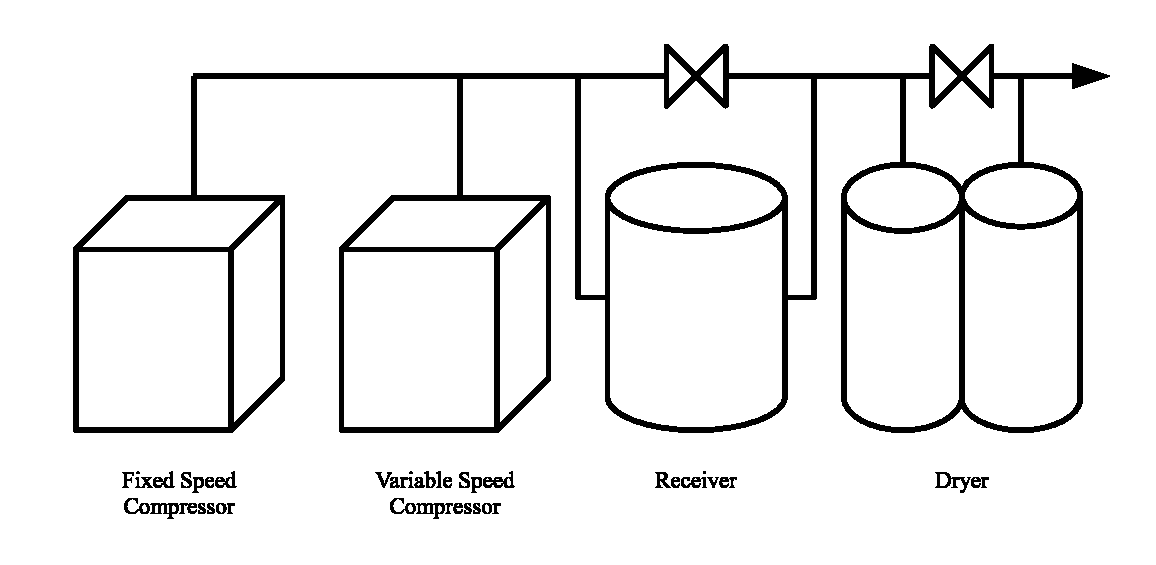
\includegraphics[width = 0.5\columnwidth]{./Images/PharmacyCompAir.eps}
\caption{Test Site Compressed Air System Layout}
\label{fig:compairlayout}
\end{figure}

\begin{figure}
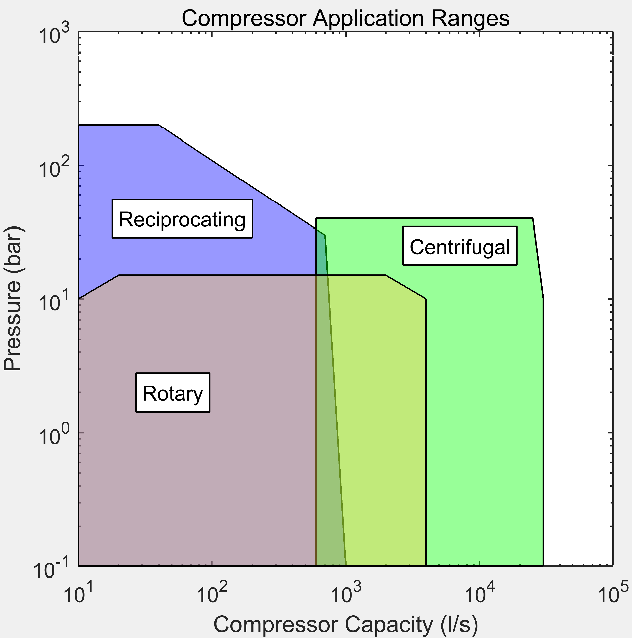
\includegraphics[width = 0.5\columnwidth]{./Images/CompApps.pdf}
\caption{Compressor Application Suitability}
\label{fig:CompApps}
\end{figure}

\begin{figure*}
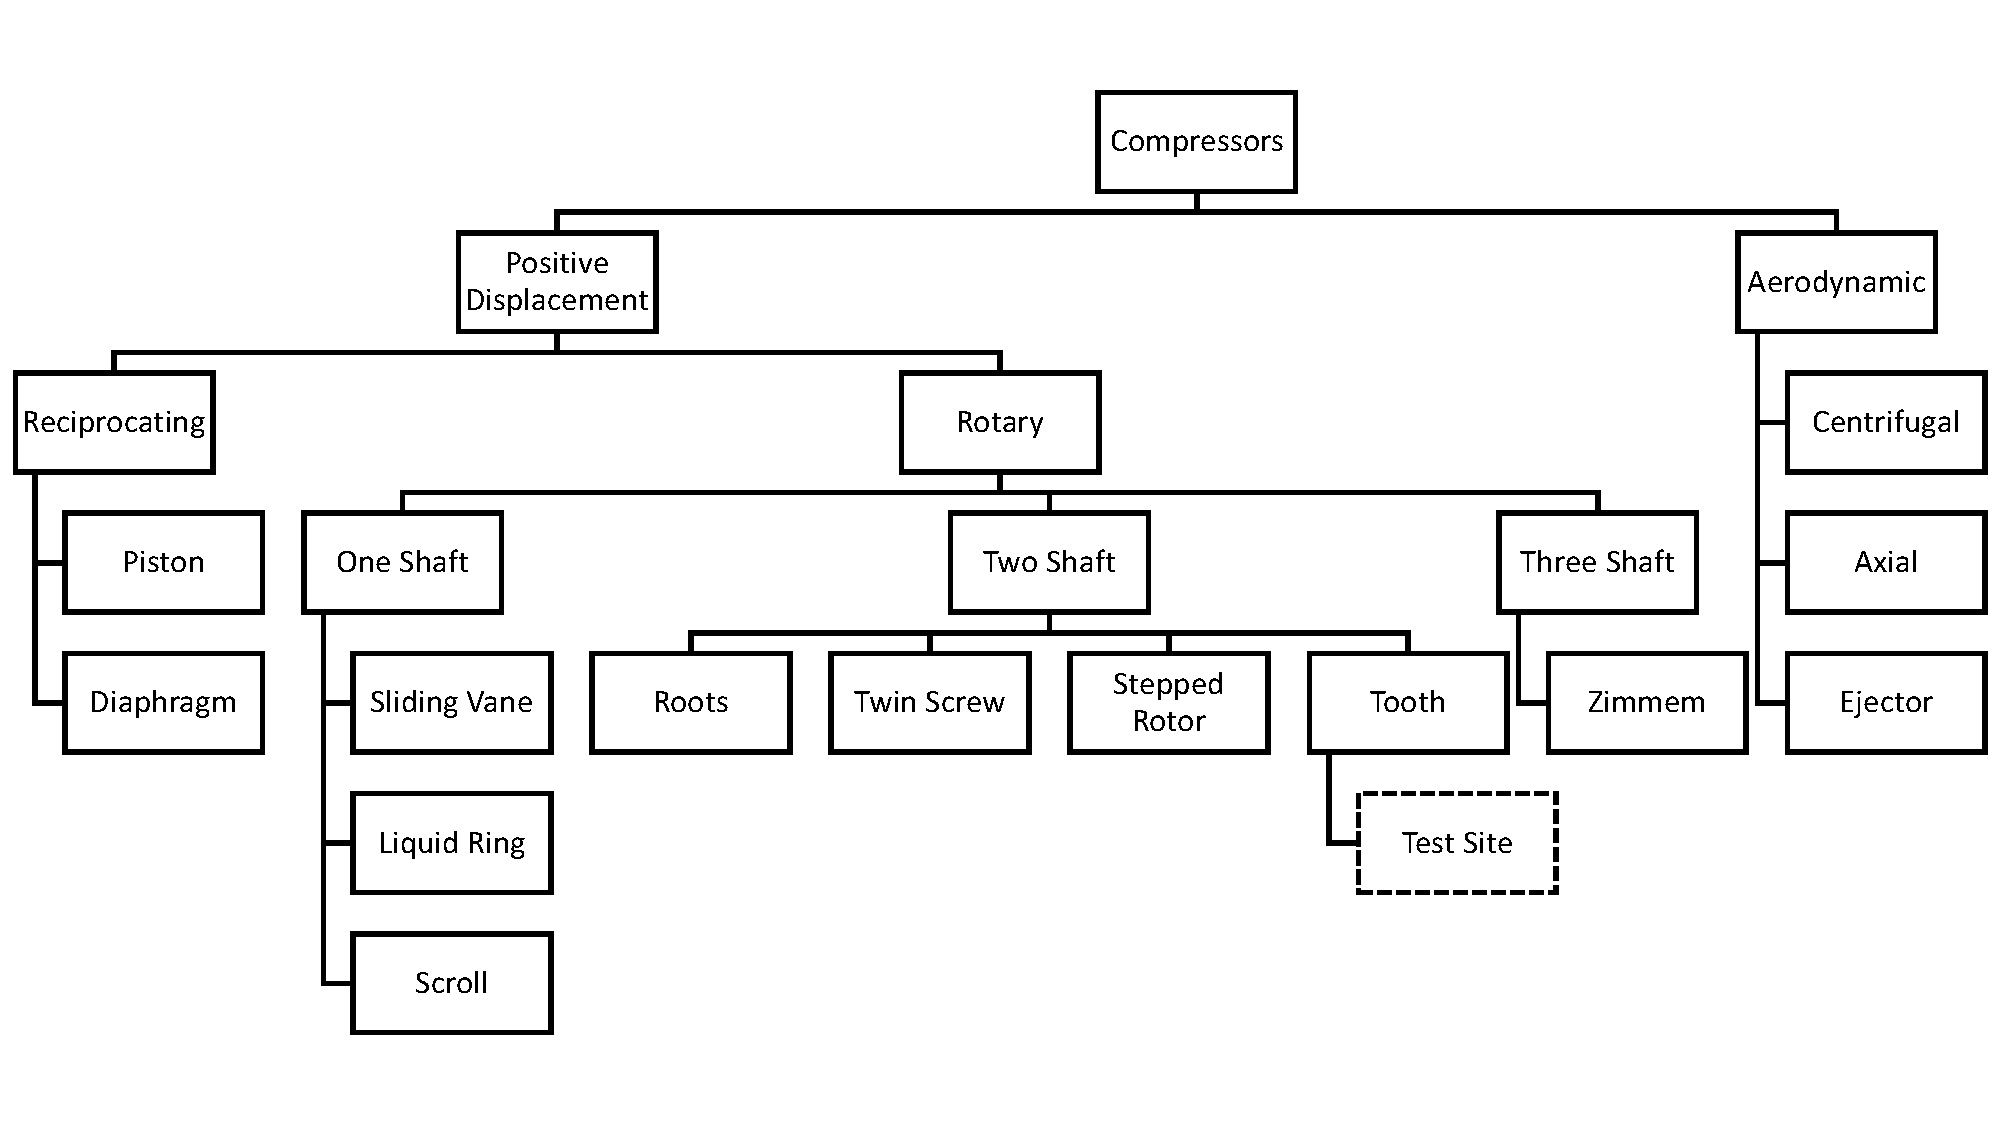
\includegraphics[width = \textwidth]{./Images/CompressorClassification.pdf}
\caption{Compressor Types}
\label{fig:comptypes}
\end{figure*}

%\subsection{Current research into performance management}
%\label{subsec:perfmgmtmethods}

Research is being carried out to define the future of compressed air system performance management, with a representative sample comprising \cite{DapengNiu2011}, \cite{Ren2012} and \cite{Kopanos2015}. In this paper the research considered is that of ongoing analysis of compressed air system data. This ongoing analysis could be designated as having any of the higher level goals outlined in \autoref{tab:goalsmgmt}.

% Table generated by Excel2LaTeX from sheet 'Sheet2'
\begin{table}
  \centering
  \caption{Goals of Performance Management}
    \begin{tabular}{p{.3\linewidth}p{.3\linewidth}p{.3\linewidth}}
    \toprule
    Goal  & Description & Example Work \\
    \midrule
    Fault Detection and Diagnosis & Monitor system parameters to determine when system is in fault condition and the potential reasons for the identified fault & Using vibration, pressure and current signals to diagnose valve faults for a reciprocating compressor (\cite{Tran2014}) \\
    \midrule
    Prognostics & Monitoring system parameters to determine when a component of a system will no longer perform its intended function (\cite{Vachtsevanos2006}) & Determining the remaining useful life of a gaseous circuit breaker  based on gas pressure and ambient temperature (\cite{Catterson2013}) \\
    \midrule
    Analytics & Monitoring system parameters to discover meaningful patterns which may advise on potential improvements to system operation & Determining abnormal appliance power consumption based on analysis of individual appliance’s acoustic noise (\cite{Pathak2015}) \\
    \midrule
    Automated Commissioning & Achieving, verifying and documenting that the performance of a system satisfies the current user requirement & Automatically carrying out the normal testing procedure for an air compressor by replicating the tasks normally carried out during commissioning (\cite{Mazid2008}) \\
    \midrule
    Optimisation & Improving system operation or design as measured against some defined criteria & Development of a tool which delivers an optimal design for a compressed air system based on energy and life cycle costing (\cite{Friden2012}) \\
    \midrule
    Control & Managing the operation of a system in order that operating conditions remain in line with design states and undesirable states are avoided & Development of a control algorithm for fixed speed compressors that provides the pressure control capabilities of a variable speed system while limiting energy consumption (\cite{Facchinetti}) \\
    \bottomrule
    \end{tabular}%
  \label{tab:goalsmgmt}%
\end{table}%

This paper categorises industrial utility performance management methods into three high-level classifications, which are themselves subdivided into individual methods. These three categories are:
\begin{enumerate}
\item Quantitative model based methods
\item Qualitative model based methods
\item Process history based methods
\end{enumerate}
These three categories are shown visually in \autoref{fig:perfmgmtmethods}, which is adapted from previous works on system performance management and diagnostic approaches (\cite{Katipamula2005}, \cite{Venkatasubramanian2003}, \cite{Venkatasubramanian2003a}, \cite{Venkatasubramanian2003b}, \cite{Gao2015}, \cite{Gao2015a}, \cite{Bruton2013}).


\begin{figure*}
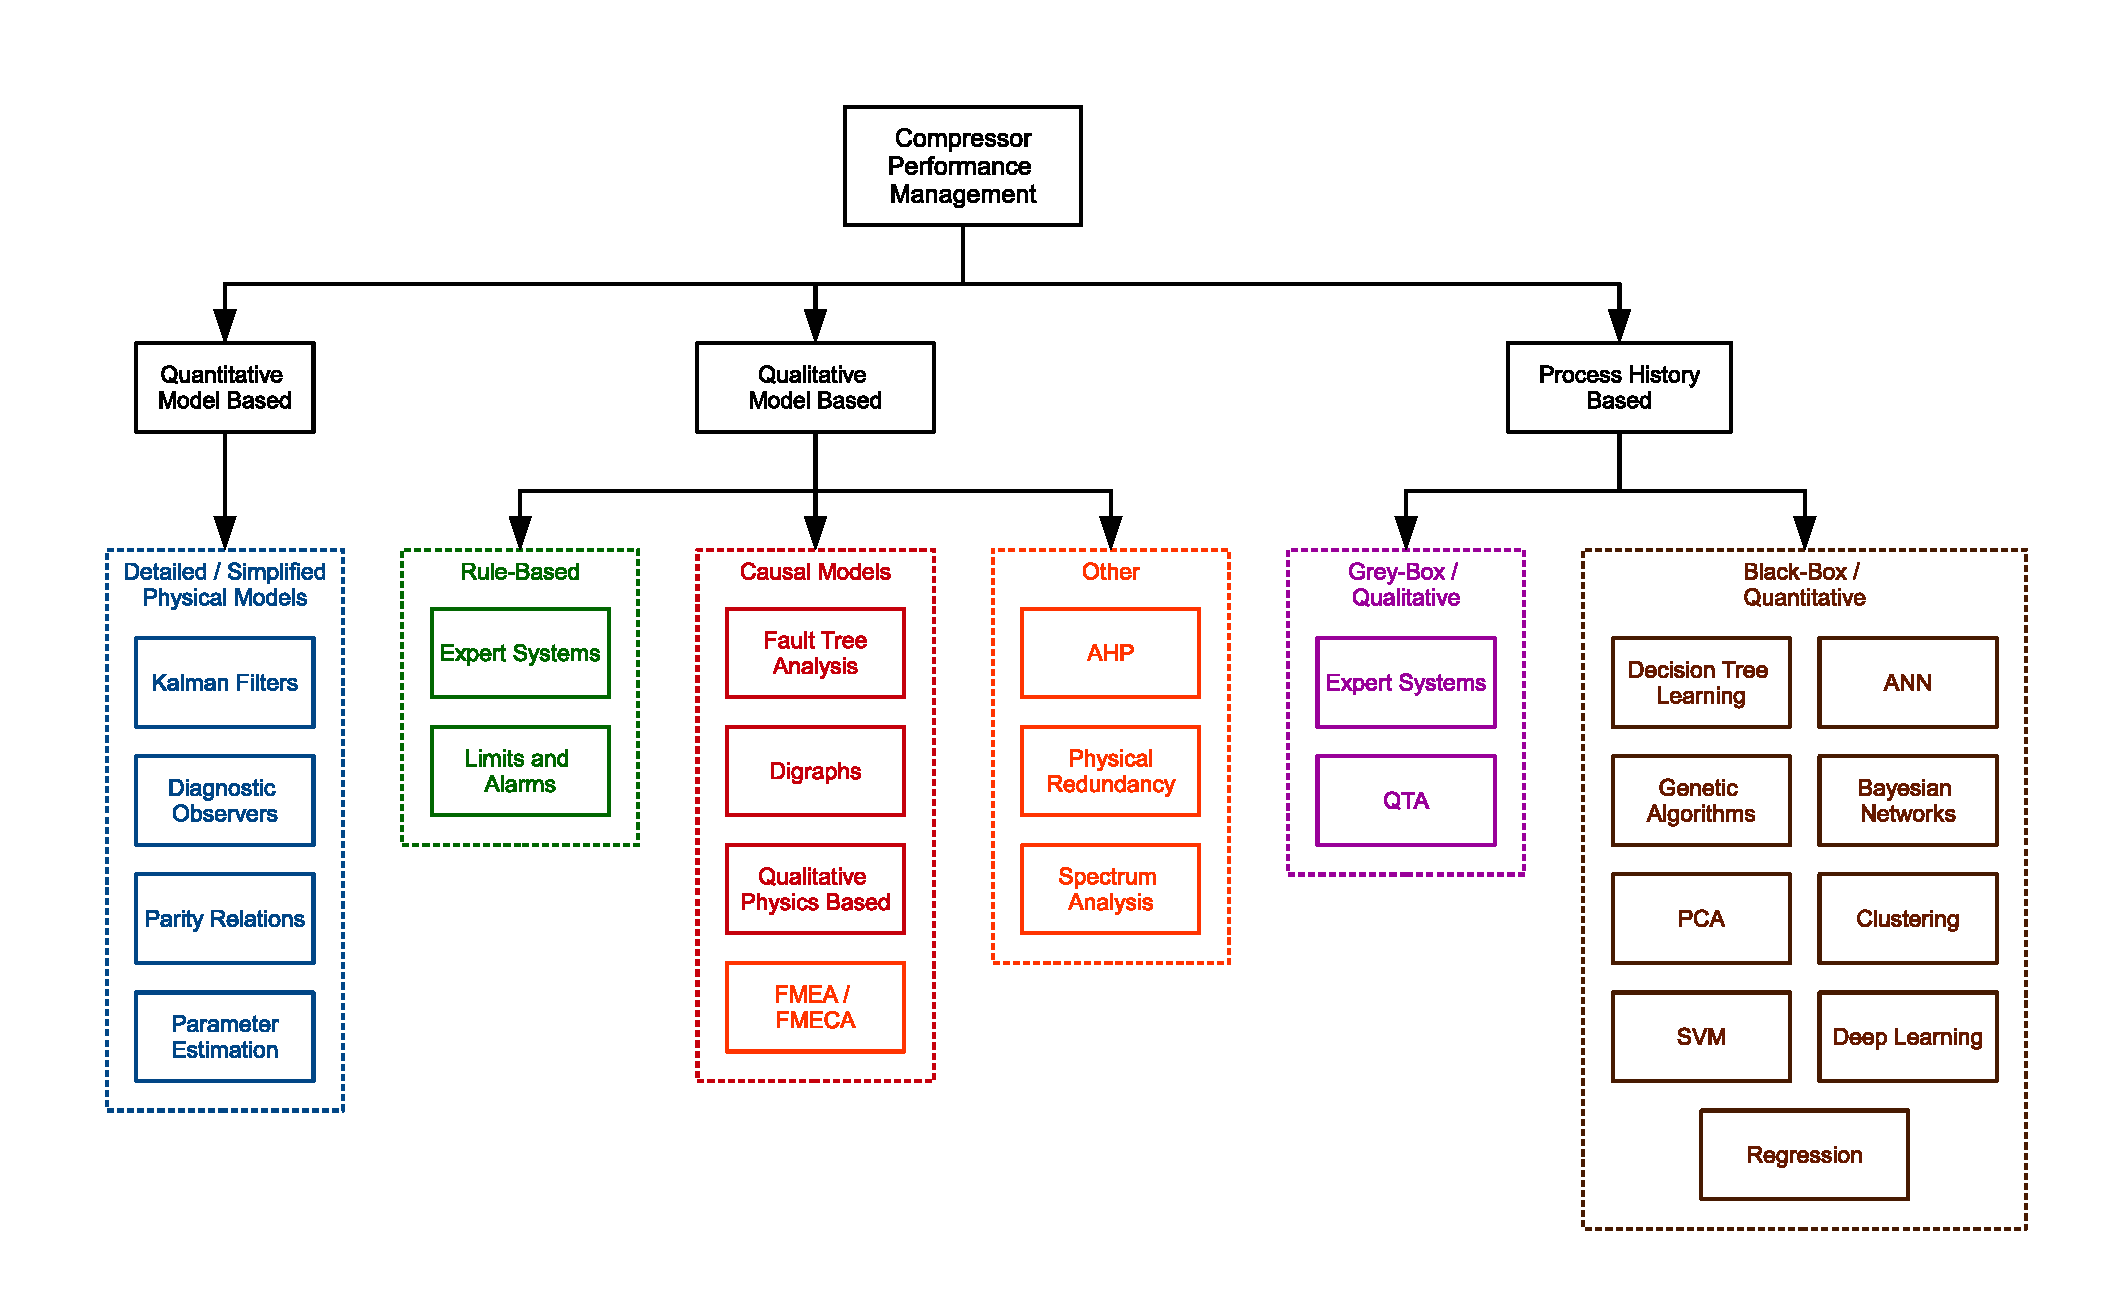
\includegraphics[width=\textwidth]{./Images/perfmgmt.eps}
\caption{Current research into performance management methods}
\label{fig:perfmgmtmethods}
\end{figure*}

\subsection{Quantitative model based methods}
In the field of compressor performance management, one approach which may be used is that of the development of a quantitative model describing the compressor's operation, and analysing actual operation with respect to this modelled operation in order to achieve one of the goals outlined in \autoref{tab:goalsmgmt}. This comparison may lead to the generation of differences between measured and modelled variables, which are termed residuals. This concept of inconsistency between variables is known as redundancy.

Analytical or artificial redundancy is achieved through formalisation of the fundamental relationships between the states, inputs and outputs of a system. This inherent redundancy may take either a direct or a temporal approach.

A direct approach to analytical redundancy is to derive algebraic equations between different sensor measurements. If a sensor is available for a calculated value, the concept of redundancy may be used to generate a residual. If the residual exceeds a given threshold then a sensor fault may be present. In contrast, temporal redundancy is obtained by analysing the difference relationships between sensor outputs and actuator inputs. If an actuator input is intended to produce a difference between sensors, and this difference is not present, then either a sensor or actuator fault may be present. Various approaches to the generation and analysis of residuals are given in \autoref{fig:perfmgmtmethods}. Quantitative model based methods have been used with success in the field of air compressors for surge control (\cite{Backi2013}), state estimation (\cite{Nair2011})and leakage detection (\cite{Krichel2011}).

Numerical models of a system have also been used with success to analyse the potential benefits to be achieved by retrofitting measures (\cite{Murray2012}, \cite{Murray2014}).


\subsection{Qualitative model based methods}
\label{subsec:qualimodel}
Qualitative model based methods may be distinguished from quantitative model based methods by their abstraction of the physical principles governing the operation of a system. Where quantitative methods seek precise numerical values for the parameters of a system, qualitative methods are generally satisfied with simplified models of a system.

To demonstrate this difference the example of an air compressor in operation is considered. If a quantitative model is used for analysis of this system, it can require inputs of all possible system and environmental variables (voltage, current, ambient air conditions) in order to make a calculation on what the compressed air flowrate should be. A qualitative approach to this situation would be to hypothesise that with an increase in current drawn by the compressor, an increase in compressed air flowrate should also be observed. While the quantitative approach may highlight a slight decrease in performance of the machine if the expected flowrate is not met, the qualitative approach will immediately highlight a serious issue with the compressor if an increase in power does not correspond to an increase in flowrate. The time required to develop quantitative solutions is typically greater than that for qualitative solutions. This suggests that for rapid deployment of ad-hoc compressor performance management solutions, a qualitative approach may be more suitable. The ability to be deployed with minimal additional sensoring also gives a high probability of required data availability, which is an additional benefit of this type of system. Of particular note in this set of performance management methods is rule-based expert systems, which have been selected as a method to trial in this paper. Rule-based expert systems have been applied with success in the area of HVAC (\cite{Bruton2014a}). For compressed air systems, qualitative model based methods have been applied for general fault diagnosis (\cite{Liu2001}), valve failure diagnosis (\cite{RuilinLin2010}), reliability assessments (\cite{Ren2012}), and safety evaluation (\cite{Zhu2013}).

\subsection{Process history based methods}
Process history based methods may be subdivided into qualitative and quantitative categories, or grey and black-box methods respectively. Grey box methods employ a degree of prior knowledge concerning the engineering operation of a system, whereas black box methods assume no such knowledge and focus purely on patterns in data.

Process history based methods have been applied to the area of compressed air system performance management for load forecasting (\cite{Liu2013}), valve failure diagnosis (\cite{Wang2010}), general fault detection (\cite{Petkovic2012}), and overall system optimisation (\cite{Kopanos2015}).

\subsubsection{Qualitative process history based methods - expert systems}
\label{subsubsec:prochistexpert}
Expert systems as applied to the process history methodology as opposed to the qualitative model methodology are concerned with extracting useful features from historical data, and using qualitative knowledge of the relevant system to explain and make use of these features.
One example of this methodology was employed during the creation of rules in \autoref{sec:rules}. While some rules were developed using hypotheses about the compressed air system under analysis, analysis of data gathered showed that under normal conditions, the oil pressure of the air compressor rose with increasing outlet pressure, and fell with decreasing outlet pressure. While this could have been hypothesised beforehand, it was not until the data was analysed that this feature was noticed. This lead to the development of a rule to highlight when oil pressure did not track compressor outlet pressure.

The limitations associated with process history based expert systems are similar to those associated with qualitative model based expert systems. In both cases a reliance is placed on the ability of the human expert to accurately determine rules and possible fault diagnoses. In the case of the oil pressure rule described above, it is hypothesised that a potential cause of fault should the oil pressure not rise when expected be that the oil pump has failed. However it is acknowledged that this fault may be equally symptomatic of a blocked valve or a sensor failure. As the fault detection system is developed further hypotheses may be drawn which will overcome multiple symptomatic faults such as this.

\subsubsection{Quantitative process history based methods}
Quantitative methods for system fault detection seek to extract useful features from historical data in a black-box fashion. The terminology of black-box is used to denote methods which are not influenced by fundamental engineering relationships between variables, but rely on statistical and machine learning methods to extract useful features. This is distinguished from qualitative or gray-box methods which employ a modicum of understanding of the physical processes governing a system’s operation.

Quantitative methods attempt to classify or group data into useful classes through pattern recognition. These methods are generally stochastic in nature, i.e. they do not assume that the future state of the system is necessarily influenced by past and present states. This gives such methods a probabilistic aspect, or a confidence rating in how accurately they are able to predict and classify system variables.

\section{Rule base development and testing}
\label{sec:rules}

\subsection{Nomenclature for rule parameters}
\label{subsec:nomenclature}
Before discussing the development of the expert rule set concerning air compressor performance assessment, it is useful to define the naming convention used. \autoref{tab:nomenclature} gives the nomenclature used in rule development. The nomenclature was developed as part of this research, and could be deployed on similar two-stage compressor systems. The nomenclature was developed as the \textit{de facto} standard for naming conventions in cases such as this (\cite{ProjectHaystack2016}) was found to be limited in its application to air compressors. This nomenclature could be incorporated into Project Haystack should widespread deployment of the system be achieved.

% Table generated by Excel2LaTeX from sheet 'Naming Convention'
\begin{table}[htbp]
  \centering
  \caption{Nomenclature}
    \begin{tabular}{rrr}
    \toprule
    \textbf{Reference} & \textbf{Item} & \textbf{Value} \\
    \midrule
    \multicolumn{3}{c}{\textbf{Sensors}} \\
    T1    & Plant Room Temperature & - \\
    T2    & Element 1 Outlet Temperature & - \\
    T3    & Element 2 Inlet Temperature & - \\
    T4    & Element 2 Outlet Temperature & - \\
    T5    & Final Delivery Temperature & - \\
    P1    & Compressed Air Pressure in Intercooler  & - \\
    P2    & Compressed Air Final Delivery Pressure & - \\
    P3    & Compressed Air Receiver Pressure & - \\
    P4    & Oil Pressure & - \\
    P5    & Ambient Pressure & - \\
    N1    & Motor starts per 5 minutes & - \\
    K1    & Compressor power &  \\
    \multicolumn{3}{c}{\textbf{Components}} \\
    C1    & Element 1 & - \\
    C2    & Intercooler & - \\
    C3    & Element 2 & - \\
    C4    & After Cooler & - \\
    C5    & Motor & - \\
    C6    & Oil Pump & - \\
    C7    & Load/Unload Valve & - \\
    \multicolumn{3}{c}{\textbf{Expected Levels}} \\
    T6    & Plant Room Temperature & \SI{25}{\degreeCelsius} \\
    T7    & Element 1 Outlet Temperature & \SI{140}{\degreeCelsius} \\
    T8    & Element 2 Inlet Temperature & \SI{22}{\degreeCelsius} \\
    T9    & Element 2 Outlet Temperature & \SI{100}{\degreeCelsius} \\
    T10   & Final Delivery Temperature & \SI{21}{\degreeCelsius} \\
    P6    & Compressed Air Pressure in Intercooler  & \SI{2.5}{\bar} \\
    P7    & Compressed Air Final Delivery Pressure & \SI{7.25}{\bar} \\
    P8    & Compressed Air Receiver Pressure & \SI{7.25}{\bar}\\
    N2    & Motor starts per 5 minutes & 1 \\
    K2    & Compressor power idle & \SI{1.5}{\kilo \watt} \\
    K3    & Compressor maximum power unloaded & \SI{8.4}{\kilo \watt} \\
    \multicolumn{3}{c}{\textbf{Warning Levels (High)}} \\
    T11   & Plant Room Temperature & \SI{35}{\degreeCelsius} \\
    T12   & Element 1 Outlet Temperature & \SI{155}{\degreeCelsius} \\
    T13   & Element 2 Inlet Temperature & \SI{24}{\degreeCelsius} \\
    T14   & Element 2 Outlet Temperature & \SI{120}{\degreeCelsius} \\
    T15   & Final Delivery Temperature & \SI{21}{\degreeCelsius} \\
    P7    & Compressed Air Pressure in Intercooler  & \SI{2.6}{\bar} \\
    P8    & Compressed Air Final Delivery Pressure & \SI{7.6}{\bar} \\
    P9    & Compressed Air Receiver Pressure & \SI{7.6}{\bar} \\
    N3    & Motor starts per 5 minutes & 2 \\
    \multicolumn{3}{c}{\textbf{Error Thresholds}} \\
    E1    & Plant Room Temperature & \SI{5}{\degreeCelsius} \\
    E2    & Element 1 Outlet Temperature & \SI{5}{\degreeCelsius} \\
    E3    & Element 2 Inlet Temperature & \SI{5}{\degreeCelsius} \\
    E4    & Element 2 Outlet Temperature & \SI{5}{\degreeCelsius} \\
    E5    & Final Delivery Temperature & \SI{5}{\degreeCelsius} \\
    E6    & Compressed Air Pressure in Intercooler  & \SI{0.1}{\bar} \\
    E7    & Compressed Air Final Delivery Pressure & \SI{0.1}{\bar} \\
    E8    & Compressed Air Receiver Pressure & \SI{0.1}{\bar} \\
    E9    & Oil Pressure & \SI{0.1}{\bar} \\
    \bottomrule
    \end{tabular}%
  \label{tab:nomenclature}%
\end{table}%



\subsection{Rule formulation methodology}
\label{subsec:rulemethodology}

One of the approaches for performance management of air compressors outlined in \autoref{subsec:qualimodel} is that of Expert Systems. This is a qualitative method which can use rule sets to encode expert knowledge about a system for highlighting when a fault in operation is present. This method has been used with success in the case of HVAC (\cite{Bruton2014}, \cite{House2001}) and in the area of air compressors (\cite{Jiang2013}). Rules for system analysis are typically derived by taking a fundamental engineering overview of the system, and hypothesising potential rules to determine particular faults.

\autoref{fig:compairflow} shows a high level overview of the test site air compressor. The figure highlights the expected temperature changes as the compressed air is operated on by each fundamental component. These expected operations form the basis for an initial set of rules to highlight when the machine is not operating as expected. To illustrate this point the first element of compression is now analysed in detail.

\begin{figure*}
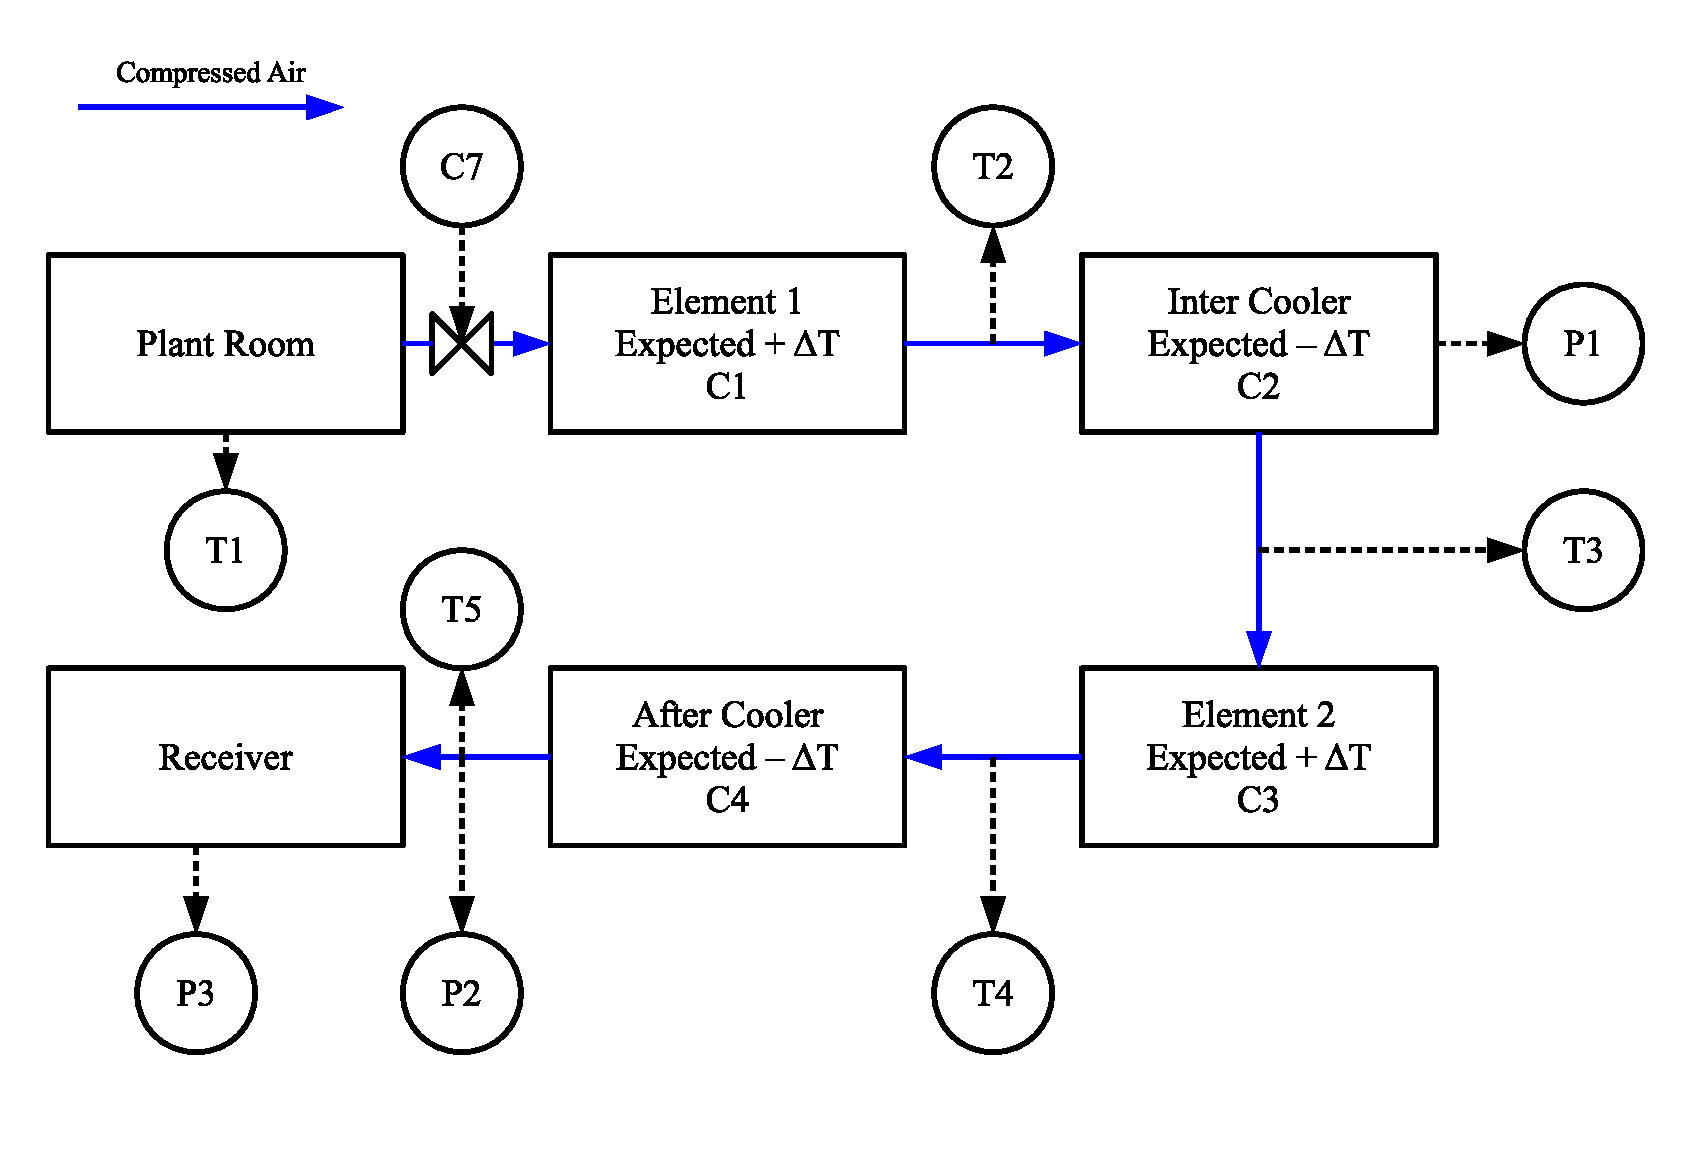
\includegraphics[width = \textwidth]{./Images/2StageRotaryCompressorIdeal.eps}
\caption{Two stage compressor air flow}
\label{fig:compairflow}
\end{figure*}

Element 1 of the air compressor compresses air from atmospheric pressure (\SI{101325}{\pascal}) to \SI{250000}{\pascal}. When the compressor is at minimum loading, it is designed to produce \SI{41}{\liter \per \second} of free air (i.e. it will draw in this quantity of air at atmospheric pressure from the plant room). It is useful to analyse the thermodynamics of compressing air at this point. \autoref{fig:thermocomp} shows the relevant thermodynamic diagrams for the compression of this volume of air isothermally, adiabatically and polytropically. The air is compressed in a space which is surrounded by ambient air, which is not an ideal heat reservoir. Therefore the isothermal compression case is not valid. The air is not however thermally isolated from its surroundings, therefore the adiabatic case is also not valid. Actual air compression typically follows the polytropic process model, with the polytropic exponent of \autoref{eq:polytropcompression} ranging between 1 and 1.4.

\begin{figure}
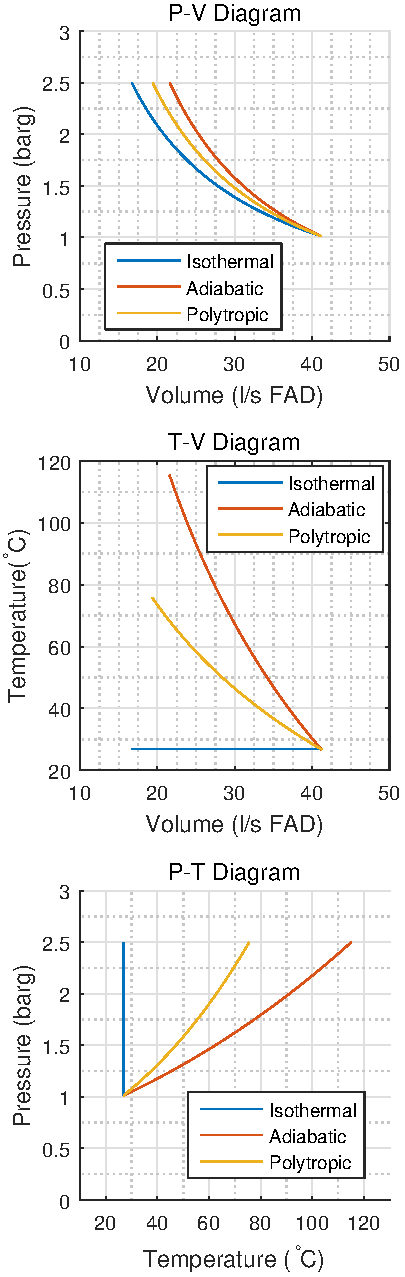
\includegraphics[height = \textheight]{./Images/Compression_ThermoDiagrams.pdf}
\caption{Thermodynamics of Air Compression}
\label{fig:thermocomp}
\end{figure}

\begin{eqnarray}
\label{eq:polytropcompression}
P_1 V_1^n = P_2 V_2^n \\
\text{where}~P = \text{Absolute pressure (Pa)} \nonumber \\
\text{V} = \text{Absolute volume (m\textsuperscript{3})} \nonumber \\ 
n = \text{Polytropic exponent} \nonumber
\end{eqnarray} 

Given that the compression process taking place is not isothermal, it is logical to expect that the temperature of the compressed air will increase through the first element of compression, in accordance with \autoref{fig:thermocomp}. If a decrease in temperature is observed, then either a failure in the first stage of compression or in a temperature sensor can be determined. This forms the basis for the first rule of the rule set created for compressor performance analysis, which is summarised in \autoref{tab:ruleset}.

\begin{equation}
\text{Rule 1. } T1 - T2 > 0
\label{eq:rule1}
\end{equation}

In a similar manner to Rule 1, Rules 2, 3 and 4 fire when the expected temperature of the compressed air does not change as expected across the intercooler, second element of compression and aftercooler respectively.

\begin{equation}
\text{Rule 2. } T3 - T2 >0
\label{eq:rule2}
\end{equation}

\begin{equation}
\text{Rule 3. } T3 - T4 >0
\label{eq:rule3}
\end{equation}

\begin{equation}
\text{Rule 4. } T5 - T4 > 0
\label{eq:rule4}
\end{equation}

Rules 5, 6, 7, 8 and 9 are threshold rules, in that they fire when defined thresholds for T1, T2, T3, T4 and T5 respectively are exceeded. These threshold values have been heuristically developed through a combination of historical data analysis and experience of the operational parameters of the system.

\begin{equation}
\text{Rule 5. } (T1-E1) > T11
\label{eq:rule5}
\end{equation}

\begin{equation}
\text{Rule 6. } (T2 - E2) > T12
\label{eq:rule6}
\end{equation}

\begin{equation}
\text{Rule 7. } (T3 - E3) > T13
\label{eq:rule7}
\end{equation}

\begin{equation}
\text{Rule 8. } (T4 - E4) > T14
\label{eq:rule8}
\end{equation}

\begin{equation}
\text{Rule 9. } (T5 - E5) > T15
\label{eq:rule9}
\end{equation}

The first element of compression in a two-stage compressor is designed to compress air to an intermediate pressure, before intercooling and compression to final delivery pressure by the second element of compression. If this intermediate pressure is not acheived, it is indicative of either a pressure sensor fault, or a fault in element 1 operation. If the first element of compression is faulty in operation, this will lead to excessive strain on the second element of compression to achieve final delivery pressure. Rule 10 highlights when this intermediate pressure is not met.

\begin{equation}
\text{Rule 10. } (P1 + E6) < P6
\label{eq:rule10}
\end{equation}

For a single compressor in isolation, if the final delivery pressure continues to rise when the compressor is running in unloaded mode, it is indicative of either a fault in the relevant pressure sensor, or that the load/unload valve of the compressor has failed. Rule 11 fires when this pressure rise in unloaded mode takes place.

\begin{equation}
\text{Rule 11. } (P2(t) - (P2(t-1)) > 0
\label{eq:rule11}
\end{equation}

If the motor driving the compressor is switching on and off excessively, it will lead to premature wear and tear on the compressor mechanical drive. Rule 12 fires when a threshold for the number of motor starts has been exceeded.

\begin{equation}
\text{Rule 12. } \sum_{t = 0}^{300s}N1 > N2
\label{eq:rule12}
\end{equation}

\autoref{fig:mechcompressor} shows the mechanical layout of a two stage air compressor. In an air compressor lubricated by oil, the oil should circulate when the compressor is loaded. If the oil pressure does not rise with the compressor loaded, it is indicative of a blockage or leakage in the oil circulation system, a failure of the oil pump, or a pressure sensor fault.

\begin{equation}
\text{Rule 13. }(P4(t) + E9) < P4(t-1)
\label{eq:rule13}
\end{equation}

\begin{figure}
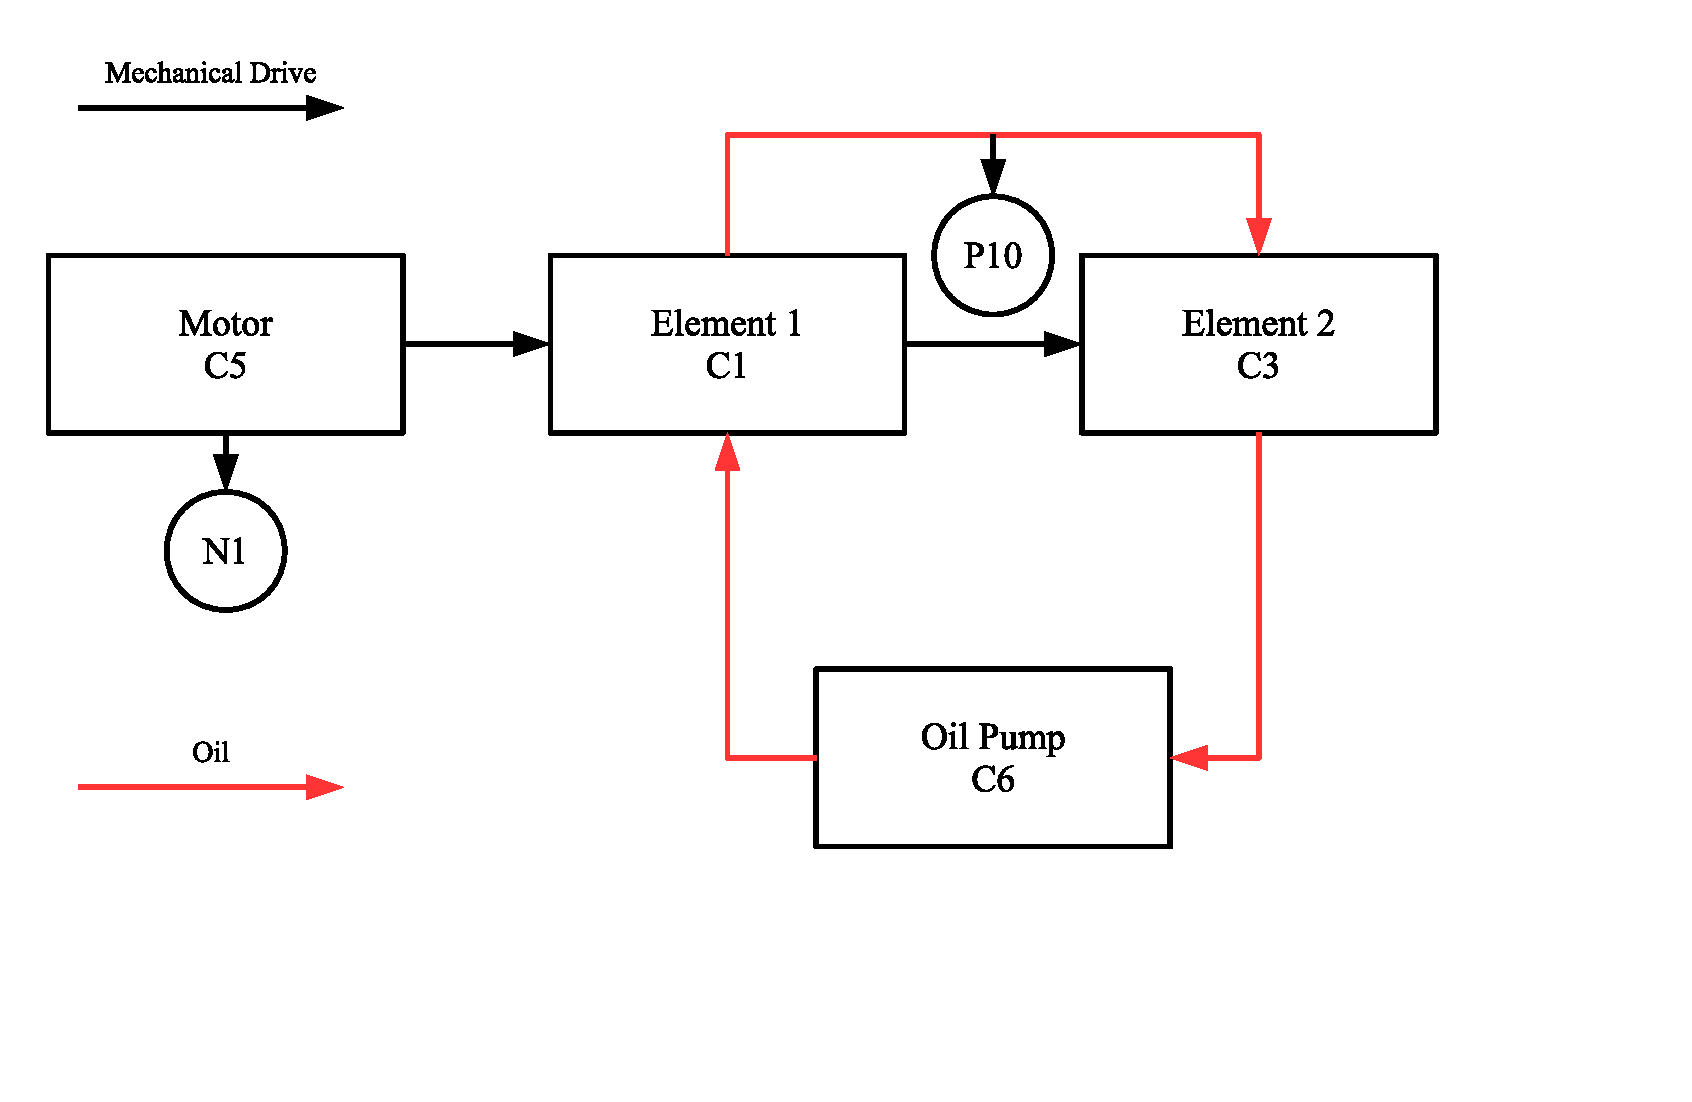
\includegraphics[width = .6\columnwidth]{./Images/MechanicalCompressor.eps}
\caption{Mechanical drive two stage compressor}
\label{fig:mechcompressor}
\end{figure}

The compression of air in both the first and second element of a two-stage air compressor follows defined thermodynamic principles. The temperature rise of compressed air for each of the three types of compression is given in \autoref{fig:thermocomp}. The theoretical maximum temperature rise of air under compression is given by the adiabatic case. Therefore, while it is known that the air will compress polytropically, it can be assumed that if the outlet temperature of either the first or second element of compression is greater than that dictated by the adiabatic case (with the polytropic exponent of \autoref{eq:polytropcompression} set to 1.4), then a fault is present in the system. This fault may either be in one of the relevant temperature sensors, or additional heat may be being supplied to the air under compression. This principle dictates when Rules 14 and 15 are fired.

\begin{equation}
\text{Rule 14. } T2 > T1 * \left(\frac{P1}{P5}\right)^\frac{\gamma-1}{\gamma}
\label{eq:rule14}
\end{equation}

\begin{equation}
\text{Rule 15. } T4 > T3 * \left(\frac{P2}{P1}\right)^\frac{\gamma-1}{\gamma} \\
\label{eq:rule15}
\end{equation}
$\text{where } \gamma = \text{heat capacity ratio of air (1.4)}$

Rules 1-15 are summarised in \autoref{tab:ruleset}, along with the potential faults which would explain each rule being fired. The potential impact on system performance of each rule being fired is given in \autoref{tab:ruleimpact}.

  
% Table generated by Excel2LaTeX from sheet 'Sheet1'
\begin{table*}[htbp]
  \centering
  \scriptsize
  \caption{Compressor performance assessment rule set}
    \begin{tabular}{r|l|r|r|r|r|r|r|r|r|r|r|r|r|r|r|r|r}
    \toprule
    \multicolumn{2}{c}{Rules} & \multicolumn{16}{c}{Potential Faults} \\
    \midrule
    ID    & Description & T1    & T2    & T3    & T4    & T5    & P1    & P2    & N1    & P10   & C1    & C2    & C3    & C4    & C5    & C6    & C7 \\
    \midrule
    1     & Element 1 Temperature Decrease & X     & X     &       &       &       &       &       &       &       & X     &       &       &       &       &       &  \\
    2     & Intercooler Temperature Increase &       & X     & X     &       &       &       &       &       &       &       & X     &       &       &       &       &  \\
    3     & Element 2 Temperature Decrease &       &       & X     & X     &       &       &       &       &       &       &       & X     &       &       &       &  \\
    4     & Aftercooler Temperature Increase &       &       &       & X     & X     &       &       &       &       &       &       &       & X     &       &       &  \\
    5     & Plant Room Temperature High & X     &       &       &       &       &       &       &       &       &       &       &       &       &       &       &  \\
    6     & Element 1 Outlet Temperature High &       & X     &       &       &       &       &       &       &       & X     &       &       &       &       &       &  \\
    7     & Element 2 Inlet Temperature High &       &       & X     &       &       &       &       &       &       &       & X     &       &       &       &       &  \\
    8     & Element 2 Outlet Temperature High &       &       &       & X     &       &       &       &       &       &       &       & X     &       &       &       &  \\
    9     & Final Outlet Temperature High &       &       &       &       & X     &       &       &       &       &       &       &       & X     &       &       &  \\
    10    & Expected Intercooler Pressure not Achieved &       &       &       &       &       & X     &       &       &       & X     &       &       &       &       &       &  \\
    11    & Increase in Outlet Pressure when Unloaded &       &       &       &       &       &       & X     &       &       &       &       &       &       &       &       & X \\
    12    & High Stop-Start Frequency of Motor Observed &       &       &       &       &       &       &       & X     &       &       &       &       &       & X     &       &  \\
    13    & Failure of Oil Pressure to Rise under Loading &       &       &       &       &       &       &       &       & X     &       &       &       &       &       & X     &  \\
    14    & Theoretical Element 1 Temperature Rise Exceeded &       & X     &       &       &       &       &       &       &       & X     &       &       &       &       &       &  \\
    15    & Theoretical Element 2 Temperature Rise Exceeded &       &       &       & X     &       &       &       &       &       &       &       & X     &       &       &       &  \\
    \bottomrule
    \end{tabular}%
  \label{tab:ruleset}%
\end{table*}%

% Table generated by Excel2LaTeX from sheet 'RuleImpact'
\begin{table}[htbp]
  \centering
  \caption{Impact of rules on compressor performance}
    \begin{tabular}{p{.1\columnwidth}p{.2\columnwidth}p{.2\columnwidth}p{.2\columnwidth}}
    \toprule
          & \multicolumn{3}{c}{Impact} \\
    \midrule
    Rule  & CA User Requirement & Energy & Maintenance / Equipment Life \\
    1     & X     &       & X \\
    2     &       & X     & X \\
    3     & X     &       & X \\
    4     &       & X     &  \\
    5     &       & X     &  \\
    6     &       & X     & X \\
    7     &       & X     & X \\
    8     &       & X     & X \\
    9     &       & X     & X \\
    10    & X     &       &  \\
    11    &       & X     & X \\
    12    &       & X     & X \\
    13    &       &       & X \\
    14    &       & X     & X \\
    15    &       & X     & X \\
    \bottomrule
    \end{tabular}%
  \label{tab:ruleimpact}%
\end{table}%

\bigskip
%\lipsum[1]

\section{Operational mode identification}
\label{sec:modeidentification}
It was noted during rule set development that it is imperative to know the mode of operation of an air compressor when applying rules. This follows on from lessons learned in similar work relating to HVAC (\cite{Bruton2014}). With an air handling unit, the different modes of operation that are useful to determine which rules to apply are Heating, Cooling with Outdoor Air, Mechanical Cooling with 100\% Air and Mechanical Cooling with Minimum Outdoor Air, with these modes further categorised into Occupied and Unoccupied Modes (\cite{House2001}). Knowing the mode of operation of equipment ensures that rules are only applied where pertinent, reducing false positive occurences.

The modes of operation designated for a variable speed air compressor are given in \autoref{tab:opmodes}. To determine which mode of operation the compressor is actually in, the power drawn by the machine was analysed. Prior information on the expected power drawn for each mode was not available from manufacturer documentation, and so a clustering methodology combined with some prior knowledge was employed.

The Compressed Air and Gas Institute (CAGI) specifies a standard data sheet for air compressors which major manufacturers adhere to (\cite{CAGI}). The input power to the compressor as given on this sheet where available is also given in \autoref{tab:opmodes}. Modes 1 and 3 were recognised as being useful modes to have knowledge of, despite not having prior knowledge of the associated input power from the CAGI data sheet. From visual observation of a power meter installed at the test site, it was noted that Mode 1 had an approximate power requirement of \SI{1}{\kilo \watt}, and Mode 3 an approximate power requirement of \SI{20}{\kilo \watt}

% Table generated by Excel2LaTeX from sheet 'Modes'
\begin{table}[htbp]
  \centering
  \caption{VSD compressor operation modes}
    \begin{tabular}{rrr}
    \toprule
    Mode  & Description & CAGI Input Power (kW)\\
    \midrule
    1     & Idle & -\\
    2     & Unloaded & 8.9 \\
    3     & Minimally Loaded & - \\
    4     & VSD 0-20\% & 27.2 \\
    5     & VSD 20-40\% & 31.2 \\
    6     & VSD 40-60\% & 38.3\\
    7     & VSD 60-80\% & 42.6 \\
    8     & VSD 80-100\% & 52\\
    \bottomrule
    \end{tabular}%
  \label{tab:opmodes}%
\end{table}%

To monitor the power drawn by the compressor for mode identification, a clustering methodology was developed. This unsupervised learning method allows the compressor power meter data to be grouped into distinct clusters as per \autoref{tab:opmodes}. An additional benefit to be gained from this approach is that a drift upward in the geometric mean or centroid of any cluster could diagnose a decrease in efficiency of the machine at that operating point, as more power is required to achieve the same output.

K-means clustering was used to group the electrical meter data into clusters. This technique groups unlabelled data into clusters where there is greater intra-group similarity than inter-group similarity. The general methodology of K-means clustering is shown in \autoref{fig:clusteroverview}. K-means clustering consists of two fundamental iterative steps preceded by one initial step. The number of clusters is set initially and denoted $k$. Centroids for the $k$ clusters are then randomly initialised. All data points are then indexed according to the cluster centroid closest to them, as shown in \autoref{eq:clustergrouping},

\begin{equation}
c^{(i)}  := \underset{k}{min}  \lVert {x^{(i)} - \mu_k} \rVert ^2 \quad \text{for} \quad i = (1, 2, ..., m)
\label{eq:clustergrouping}
\end{equation}

where $C$ is a vector of elements $c^{(i)}$ the same length as the data set $X$ with $m$ points $x^{(i)}$. The vector $C$ gives the index of the cluster centroid closest to each point in $X$.

Following this step there are $k$ clusters in the dataset $X$, each of which is a subset of the overall dataset and is denoted by $S_j$. The centroids of each cluster are recomputed as the mean of all points assigned to each cluster, as shown in \autoref{eq:centroidassign},

\begin{equation}
\mu_j := \frac{1}{|S_j|}\sum_{x_j \in S_j} x_j \quad \text{for} \quad j = (1, 2, ..., k)
\label{eq:centroidassign}
\end{equation}

where $x_j$ is a point in the dataset $X$ which is assigned to the $j^{th}$ cluster. \autoref{eq:clustergrouping} and \autoref{eq:centroidassign} are then iterated until the assignments of data points to different clusters no longer change.

\begin{figure}
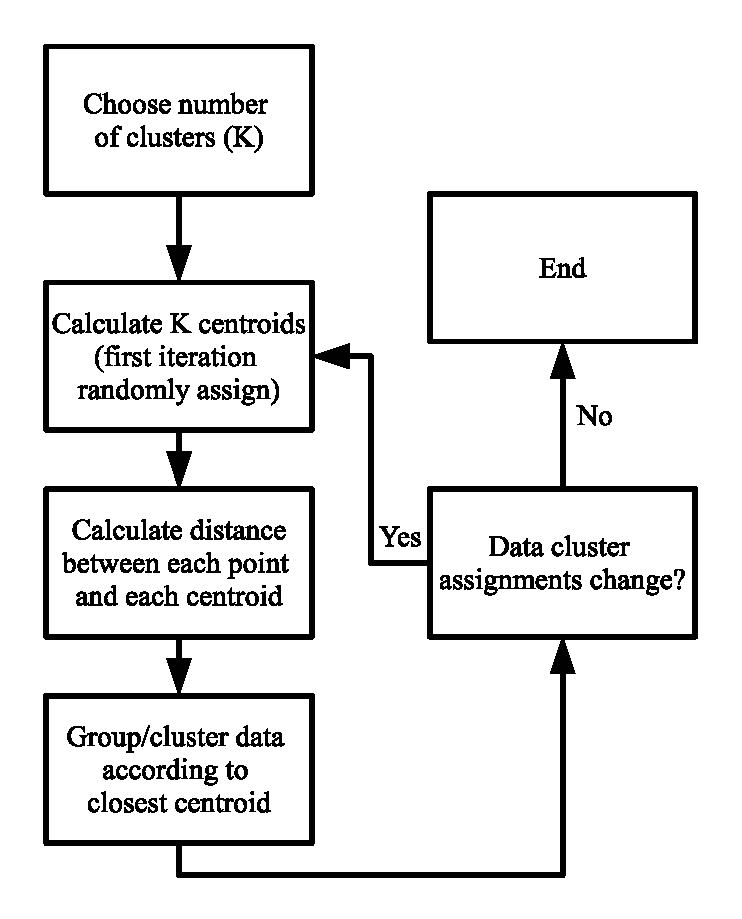
\includegraphics[width = .5\columnwidth]{./Images/ClusteringOverview.eps}
\caption{K-means clustering methodology}
\label{fig:clusteroverview}
\end{figure}

An initial attempt was made to cluster the power consumption data into two groups, i.e. Idle/Unloaded and Loaded or Modes 1-2 and 3-8 from \autoref{tab:opmodes} respectively. $k$ was therefore initially set to 2. The results of this exercise are shown in \autoref{fig:twomeansclustering}. When comparing the cluster centroids to the values in \autoref{tab:opmodes} and visual observation of the compressor power under operation, it can be determined that one of the two clusters formed is of use in further analysis, i.e. $c^{(1)} = \SI{21.3}{\kilo \watt}.$ This is a reasonable representation of the power drawn by the compressor at minimal loading. However $c^{(2)} = \SI{7.2}{\kilo \watt}$ is not as useful a value, as it is clear from \autoref{fig:twomeansclustering} that the cluster centroid is significantly below the clear cluster of compressor power operating in unloaded mode.

\begin{figure}
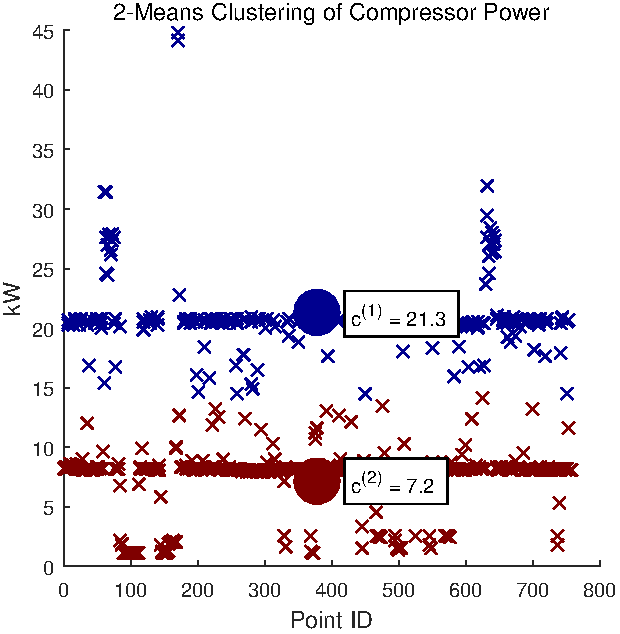
\includegraphics[width = .5\columnwidth]{./Images/2MeansClustering.pdf}
\caption{2-Means Clustering Results}
\label{fig:twomeansclustering}
\end{figure}

In order to try to gain more useful information about compressor power at different operating modes, $k$ was increased to 3. The intention was that the clear distortion of $c^{(2)}$ by the grouping of compressor power in idle mode at approximately \SI{1}{\kilo \watt} be removed by forming a new cluster for idle mode or Mode 1 as per \autoref{tab:opmodes}. The results of this exercise are shown in \autoref{fig:3meansclustering}. Mode identification is accurate with this approach for Modes 1, 2 and 3 as per \autoref{tab:opmodes}, as the cluster centroids are consistent with both known and observed values for the different modes.

\begin{figure}
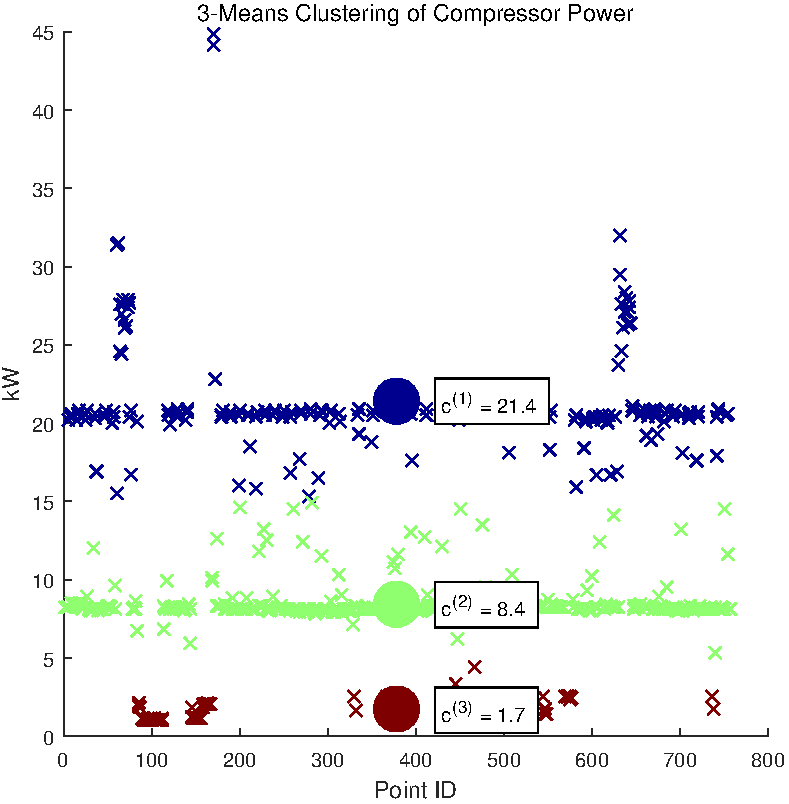
\includegraphics[width = .5\columnwidth]{./Images/3MeansClustering.pdf}
\caption{3-Means Clustering Results}
\label{fig:3meansclustering}
\end{figure}

The ideal level of accuracy for mode identification would be to determine cluster centroids for each of Modes 1-8. However the test site air compressors are significantly oversized compared to the compressed air demand. It was known that at no point in the training set did the compressor operate in Mode 8, and very rarely operated in Modes 4-7. Therefore a 7-means clustering approach was implemented. The results of this analysis are shown in \autoref{fig:7meansclustering}. When comparing the results with \autoref{tab:opmodes}, it is clear that there are two superfluous clusters in the region between Modes 2 and 3. That the analysis was unable to identify cluster centroids for Modes 5 and 6 is attributable to two factors. Firstly, there is a very low incidence of data points in these operating modes in the data set used. Secondly, the compressor takes a number of seconds to ramp up or down between Modes 2 and 3. The relatively high granularity of the data set (recording every 10 s) meant that a reasonably significant number of data points are recorded between these modes, and so the superfluous clusters have been identified.

\begin{figure}
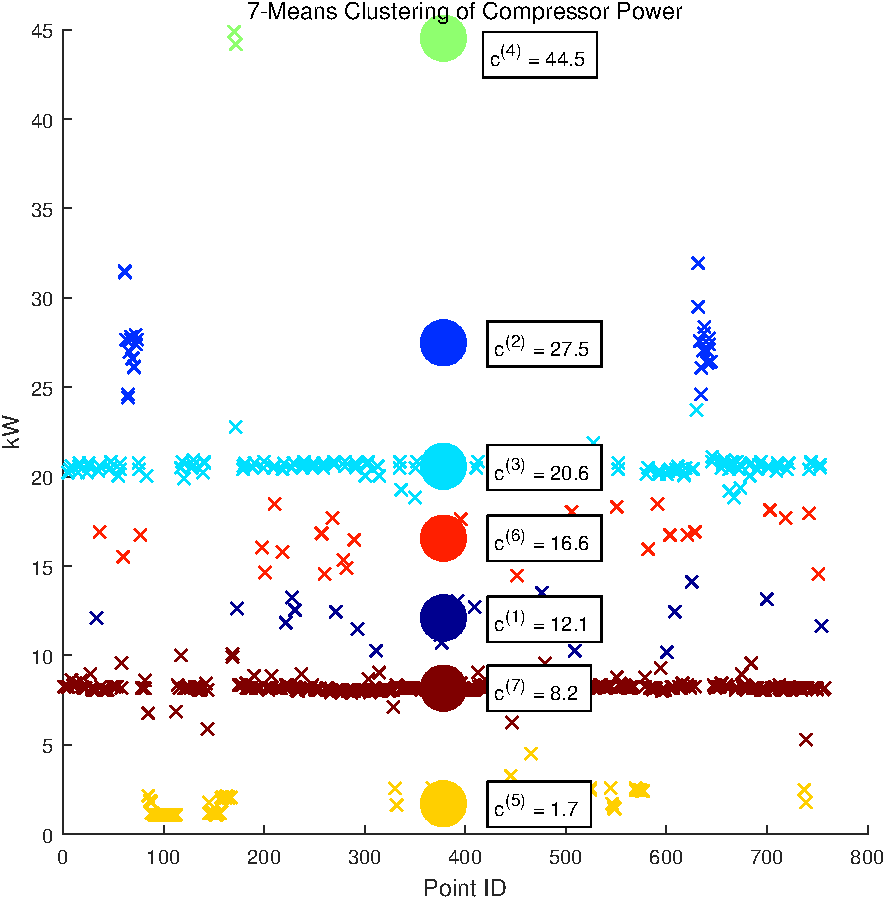
\includegraphics[width = .5\columnwidth]{./Images/7MeansClustering.pdf}
\caption{7-Means Clustering Results}
\label{fig:7meansclustering}
\end{figure}

While the 7-means clustering exercise identified superfluous clusters, it demonstrated that for the test case data set clustering was able to effectively identify five modes of operation. Therefore 5-means clustering was implemented on the data set to group the data into operational modes 1-4 and 7. The results of this implementation are shown in \autoref{fig:5meansclustering}. As expected this approach was able to correctly group the data into the required operational modes as per \autoref{tab:opmodes}.

\begin{figure}
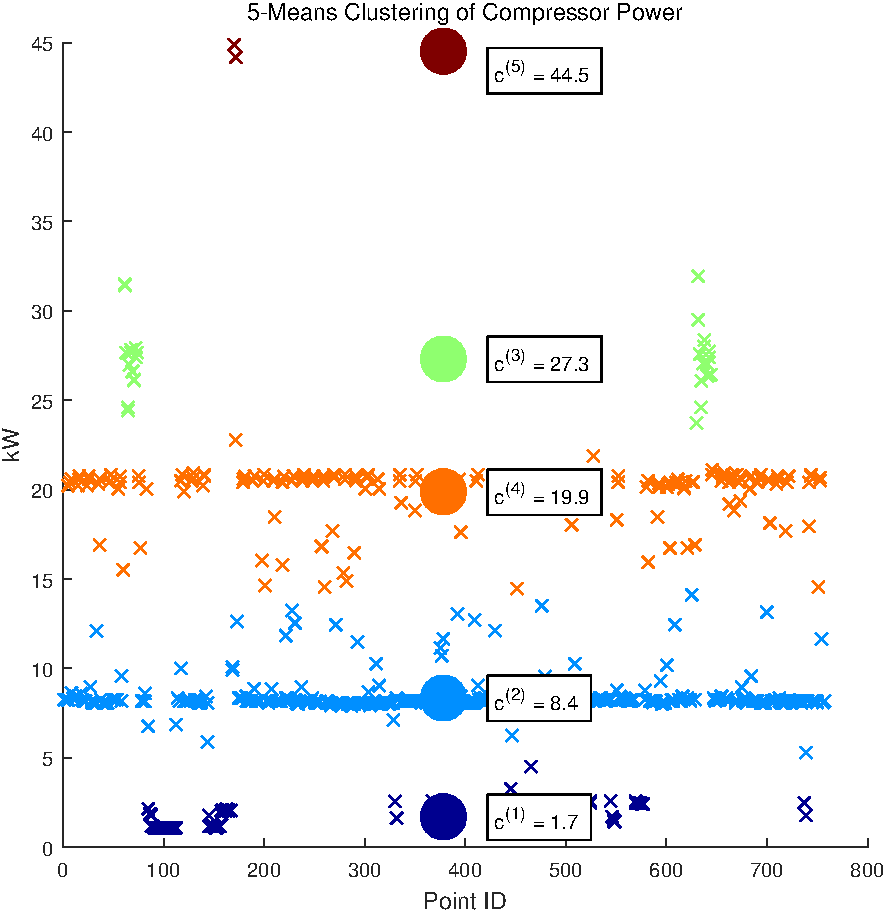
\includegraphics[width = .5\columnwidth]{./Images/5MeansClustering.pdf}
\caption{5-Means Clustering Results}
\label{fig:5meansclustering}
\end{figure}

The clustering method for mode identification was used to apply rules only when pertinent. The applicability of rules to different modes of operation is given in \autoref{tab:modeapplication}.

% Table generated by Excel2LaTeX from sheet 'ModeApplication'
\begin{table}[htbp]
  \centering
  \caption{Rule applicability of modes}
    \begin{tabular}{r|rrr}
    \toprule
          & \multicolumn{3}{c}{Mode} \\
    \midrule
     Rule & 1     & 2     & 3:8 \\
     \midrule
    1     &       &       & X \\
    2     &       &       & X \\
    3     &       &       & X \\
    4     &       &       & X \\
    5     & X     & X     & X \\
    6     &       &       & X \\
    7     &       &       & X \\
    8     &       &       & X \\
    9     &       &       & X \\
    10    &       &       & X \\
    11    &       & X     &  \\
    12    &       &       & X \\
    13    &       &       & X \\
    14    &       &       & X \\
    15    &       &       & X \\
    \bottomrule
    \end{tabular}%
  \label{tab:modeapplication}%
\end{table}%


\subsection{Mode application to efficiency monitoring}
\label{subsec:modeefficiency}
A useful application of the 5-means clustering method utilised would be to detect when the efficiency of the air compressor deteriorates. This could be achieved by continually updating the cluster centroids with new data and monitoring if there is an increase in power consumption for any given mode. The results of this approach are shown in \autoref{fig:efficiencymonitoring}. It was observed visually during the recording period that the compressor did not cover the operational range from Modes 1-7  until approximately the 175th recording (approximately \SI{0.5}{\hour}), which accounts for the clear initial training period with instability in cluster centroids. 

There is a slight increase in power consumption for Mode 1 which may be attributable to an increase over time in the cooling of the power electronics associated with the variable speed drive controller. Future work will monitor these cluster centroids over a longer time span, allowing for concrete determination of when the power usage of the compressor is excessive compared to historical data. The effectiveness of tracking performance metrics such as this has been demonstrated as being powerful for improving a building's operation (\cite{OSullivan2004}).

\begin{figure}
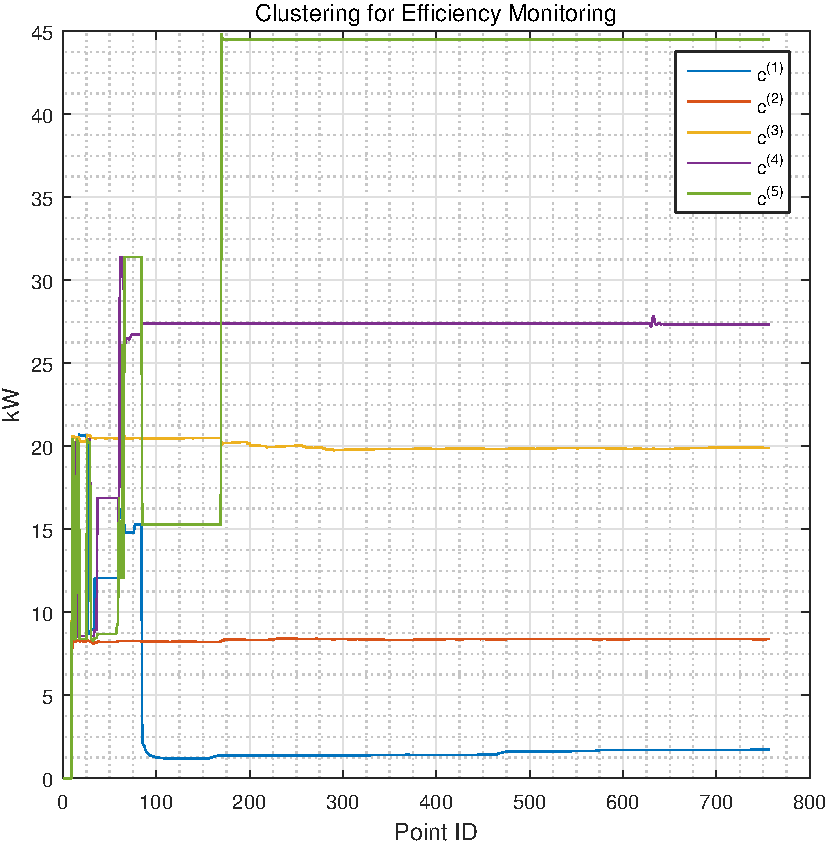
\includegraphics[width = .5\columnwidth]{./Images/EfficiencyDegradation.pdf}
\caption{Clustering for efficiency monitoring}
\label{fig:efficiencymonitoring}
\end{figure}

\section{Fault detection implementation}
\label{sec:results}

In practice several key steps are taken to implement an operational performance management methodology. These steps are outlined in \autoref{fig:implementationsteps}. Currently the initial two steps of the methodology have been implemented. Actual operational data is drawn manually and used as a static test for the system. Future work is planned to automate the data extraction process, and to refine the methods used for improved fault detection accuracy.

\begin{figure}
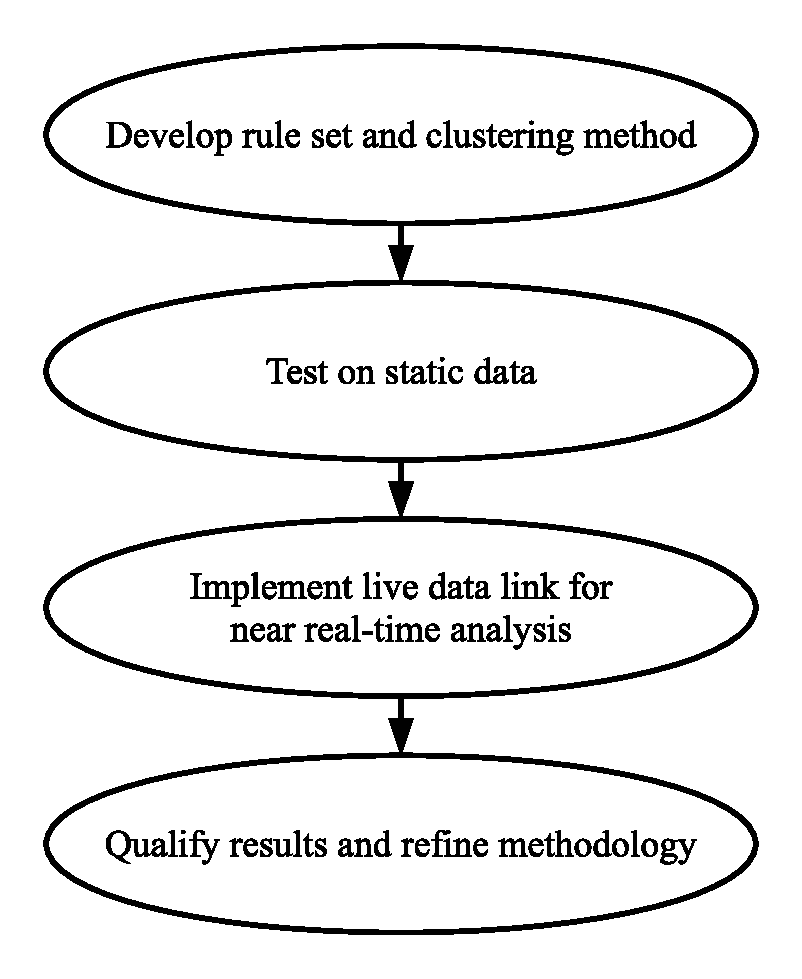
\includegraphics[width = .5\columnwidth]{./Images/ImplementationSteps.eps}
\caption{Operational performance management implementation steps}
\label{fig:implementationsteps}
\end{figure}

\subsection{Data extraction}
In order to apply the compressor performance rule set it was required to extract the operational data from the test site air compressors. A Modbus network was created to achieve this goal. The Modbus network daisy-chains the two air compressors on site with the compressed air dryer. A proprietary gateway exposes the Modbus registers of the 50 key performance parameters required for analysis. This gateway is supervised by a Tridium JACE box which acts as a Modbus master. The JACE box is connected to the internet using a 4G mobile modem, which allows for remote access and download of operational data. The overall flow of data extraction from the compressed air network to analysis by MATLAB is shown in \autoref{fig:dataflow}. A screenshot of the web interface of the JACE box is shown in \autoref{fig:jacescreen}.


\begin{figure}
\includegraphics[width = .5\columnwidth]{./Images/DataFlowArchitecture.eps}
\caption{Data Flow Architecture}
\label{fig:dataflow}
\end{figure}

\begin{figure*}
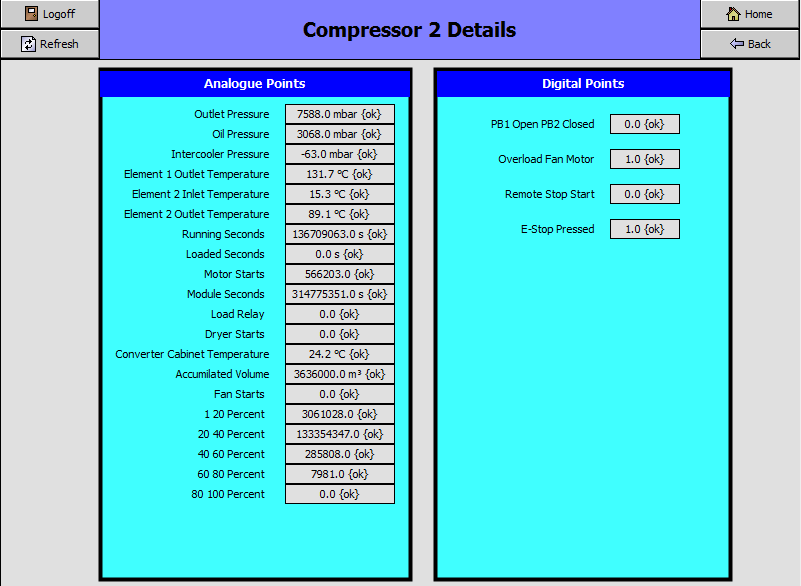
\includegraphics[width = 0.9 \textwidth]{./Images/JACE_Screen.png}
\caption{Screenshot of compressed air monitoring system}
\label{fig:jacescreen}
\end{figure*}


\subsection{Rule set and clustering implementation}
The data which was extracted from the compressed air monitoring system was stored in a MySQL database, to allow for analysis using MATLAB. Clustering was used to determine the operational mode of the air compressor at any given point. This knowledge was then used to apply pertinent rules to the data as per \autoref{tab:modeapplication}. To allow for visualisation of the knowledge gained from the analysis a GUI was created. A screenshot of this GUI is shown in \autoref{fig:ruletester}, with testing of rule 14 shown for demonstration purposes. The top section of the GUI displays operational data relevant to the rule being checked. The lower section shows the status of the rule being checked. A value of 1 denotes that the rule has fired, and 0 that there is no issue. Each rule was tested against the test case data set using this GUI. Of the 15 rules, nine (Rules 7-15) were found to recurrently highlight a fault in operation for the test data set. Each of these 9 fault symptoms indicates one of a possible two root causes. Manual verification of which is the actual cause of fault is therefore required at this stage. Future refinement of the rule set is planned to definitively diagnose the root cause for these multi-symptomatic faults. Rule 14 is now analysed in detail.

It is clear that in the case of rule 14, the rule fires frequently. This suggests either that the compressed air is picking up heat in excess to the heat of compression, or that a sensor is faulty. Given that the rule does not fire continuously, a sensor fault may be ruled out. Therefore the compressed air is picking up excess heat during compression, likely from friction of moving parts close to the compression chamber. This could be verified by inspection of the machine by a service engineer. The GUI developed and shown for Rule 14 may be used for continual analysis of the compressor performance to allow for intelligent recommendations as to when the compressor is operating sub-optimally.

\begin{figure*}
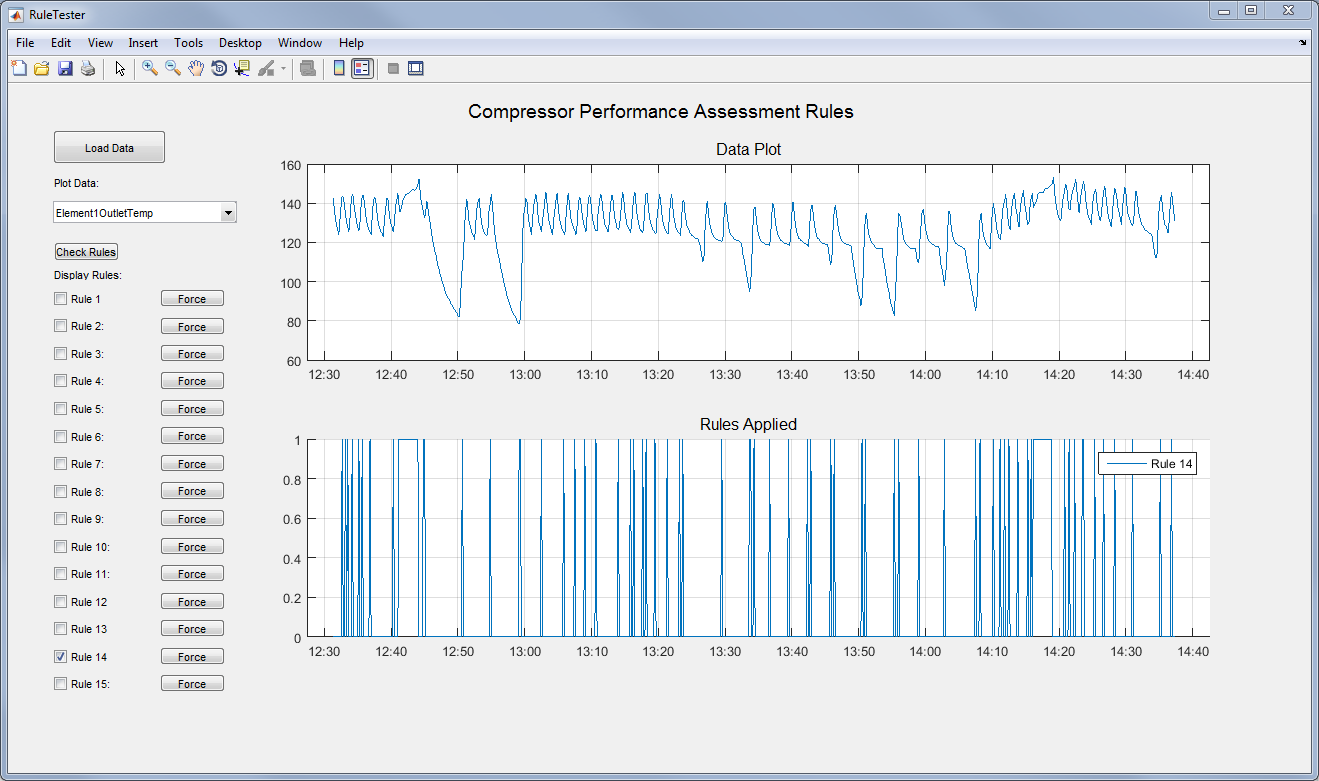
\includegraphics[width = 0.9\textwidth]{./Images/RuleTester.png}
\caption{Screenshot of compressor performance assessment GUI}
\label{fig:ruletester}
\end{figure*}


\section{Conclusions and future work}
\label{sec:conclusions}
A rule based expert system has been created for fault detection of an industrial compressed air system. The expert system employs k-means clustering for mode identification and improved energy efficiency monitoring. Implementation has been achieved using MATLAB, with results demonstrated using a custom-built GUI.

The methodology was able to successfully detect faults on a static data set. The threshold rules were developed heuristically from experience. Further refinement as more data becomes available would be advantageous for having greater confidence in these values.

It was found that the necessary data for implementation of the methodology was readily available using the Modbus capabilities of the air compressors. The test case air compressors are of a widely used make and are reasonably old. It can be expected therefore that this data will be readily available if the methodology were to be rolled out on a wider basis across industry. 

The fact that the test site air compressors are oversized meant that their full operational range was not exercised. This limited the effectiveness of the K-means clustering methodology for mode identification. In practice it would be desirable to force the compressed air system to operate over a wide capacity range to improve the methodology's mode identification capabilities.

Currently each of the 15 rules has two or more potential diagnoses. Further refinement of the existing rule set of 15 rules would allow for definitive diagnosis of the root cause of faults. This refinement could take the form of subdivision of the existing rule set, to have a unique rule for each diagnosis. 

Rules 1-6 did not detect any faults in the test data set. While this may be the case in reality, as more data becomes available and manual inspections of the compressed air system are carried out it may be desirable to modify the error thresholds for these rules if actual faults are present in the system. The main goal of any refinement of the existing rule set is to reduce the presence of false positives or false negatives.

It is planned to automate the process of data extraction from the system Modbus network, as currently Excel sheets are required to be downloaded manually and added to the tool's MySQL database. As more data is added to the system, an analysis of the energy efficiency performance will be carried out using real-time updates to the operational mode cluster centroids. To ensure that this work is scalable across multiple facilities a best-practice approach will be taken, applying the methodology of an industrial big data pipeline (\cite{ODonovan2015a}). Quantification of the financial savings achieved by implementing recommendations made by the expert system will also be carried out, taking a cost-benefit approach toward analysis (\cite{Walsh2013}).


\begin{acknowledgements}
Thanks are extended to the School of Pharmacy at University College Cork for allowing the building compressed air system to be used for trial purposes. This work was funded by Marine Renewable Energy Ireland (MaREI) at University College Cork.
\end{acknowledgements}
%\newpage
% BibTeX users please use one of
\bibliographystyle{spbasichayes}   % basic style, author-year citations
%\bibliographystyle{spmpsci}      % mathematics and physical sciences
%\bibliographystyle{spphys}       % APS-like style for physics
\bibliography{JournalPaper1E.bib}   % name your BibTeX data base

% Non-BibTeX users please use
%\begin{thebibliography}{}
%
% and use \bibitem to create references. Consult the Instructions
% for authors for reference list style.
%
%\bibitem{RefJ}
% Format for Journal Reference
%Author, Article title, Journal, Volume, page numbers (year)
% Format for books
%\bibitem{RefB}
%Author, Book title, page numbers. Publisher, place (year)
% etc
%\end{thebibliography}

\end{document}
% end of file template.tex

